\chapter{Beheer, Validatie en Verificatie}
In dit hoofdstuk wordt er beschreven hoe er tijdens de afstudeer periode de kwaliteit bewaard is van het eindproduct.
Eerst wordt er besproken hoe de code gevalideerd is met andere developers en hoe de afstudeerstage voortgang gesprekken gingen.
Daarna wordt besproken hoe versiebeheer is aan gepakt binnen het project.
Ook wordt er besproken hoe de afstudeer opdracht proces matig is aangepakt.
Voor het valideren en verfiren van de afstudeer opdracht is er een testrapport gemaakt en zijn de requirements terug gekoppeld met de stakeholders.
\section{Codereviews}
Tijdens het development process is er gebruik gemaakt van codereviews voor zowel de frontend en backend code.
Voor de backend code is Kevin (Backend software engineer) benaderd om de code te bekijken en begeven van feedback.
Daarnaast is er samen met Thom (Senior software engineer) een keer perweek een progressie update gegeven van de developement en is daar ook veel kenis gedeelt. 


\section{Versiebeheer}
Voor versiebeheer is er gebruik gemaakt van git en als repository platform Bitbucket.


\section{Codestandaarden}
Tijdens het ontwikkelen van de afstudeeropdracht is er gecontrolleerd op de code standaarden die gebruikt zijn.
Deze controlles werden tijden de code reviews en stagevoortgang besproken (Zie sectie \ref{section:CodereviewsEnStageVoortgang}).
% Omdat Snakeware niet een vaste guideline heeft voor code standaarden is er zelf een opgesteld die gevolgt is tijdens de afstudeeropdracht.
% Deze standaarden staan vermeld in de bijlage \textbf{(bron)}.

\section{Process en bewaking}
Tijdens de afstudeerperiode is er gewerkt met een Agile \parencite{Agile} methode genaamd Scrum \Parencite{Scrum}.
Er is gewerkt met sprints van 2 weken waar bij de requirements opgedeeld werden in kleine stukjes.
Dit is gedaan om de taken behapbaar te maken en om snel veranderingen te kunnen aanbrengen.
Elke week werd er met de afstudeerbegeleider de progressie gesproken van de week waar bij mogelijk bijgestuurd werd.
De verschillende sprints werden bijgehouden in een notitie programma \textbf{Obsidian} hierbij is elke sprint opgedeeld in een apparte note.
Vervolgens is er gebruikgemaakt van een scrumboard om de progressie bij te houden dit werd ook gedaan in Obsidian.
In figuur \ref{fig:VoorbeeldSprint} is te zien hoe zo'n sprint ingepland werdt.

\whitespace[2]
\begin{graphic}
	\captionsetup{type=figure}
	\caption{Sprint 4 van het realisatie process}
	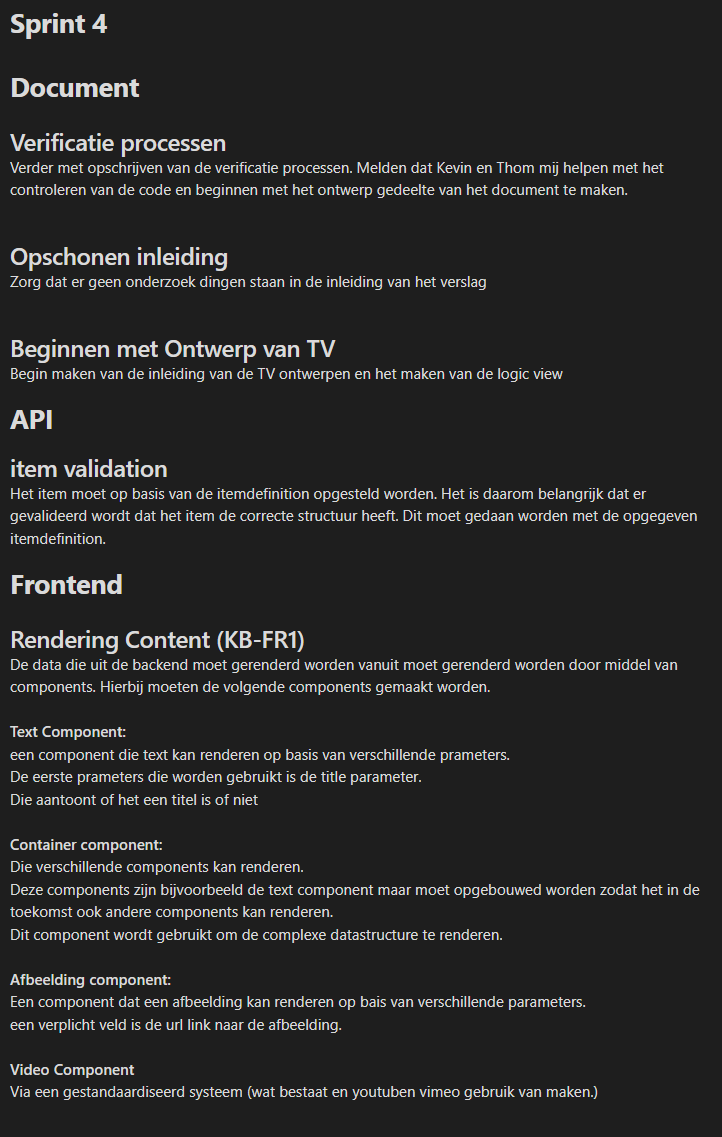
\includegraphics[scale=0.5]{SprintVoorbeeld.png}
	\label{fig:VoorbeeldSprint}
\end{graphic}

\section{Testrapport}
Tijdens het ontwikkelen van het eindproduct zijn er verschillende testen uitgevoerd.
Er is gebruik gemaakt van het V-model de Teststrategie die gebruikt wordt is beschreven in sectie \ref{section:Teststrategie}.
In dit hoofdstuk worden de verschillende testen toegelicht en behandeld.

\subsection{Unittesten}
Voor het unit testen van de API is er gebruikgemaakt van xUnit (voor meer informatie zie sectie \ref{section:Bouwomgeving}).
Unit testen worden gebruikt om de verschillende logica van het systeem te testen.
Hierom zijn testen geschreven voor de handlers en de data mappers in de applicatie.
Een voorbeeld van zo'n unit test is te zien in figuur \ref{fig:ExampleUnitTest}.
Verder is er een overzicht van de verschillende unittesten in figuur \ref{fig:OverviewUnitTests}.

\whitespace[2]
\begin{graphic}
	\captionsetup{type=figure}
	\caption{Geïmplementeerde unit test}
	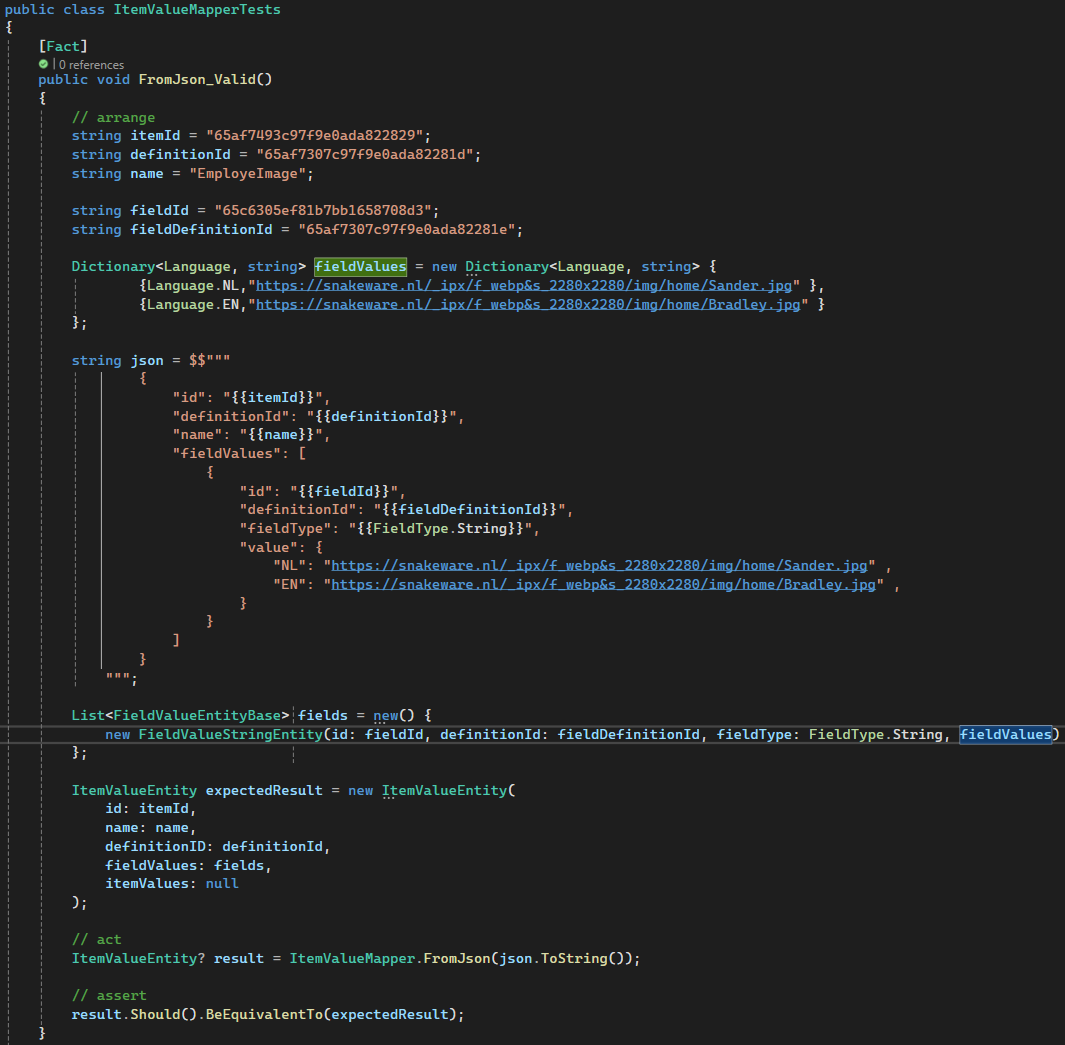
\includegraphics[scale=0.52]{ExampleUnitTest.png}
	\label{fig:ExampleUnitTest}
\end{graphic}

\subsection{Intergratietesten}

\subsection{Systeemtesten}
Voor de systeemtesten zijn de webapplicatie en API handmatig getest.
Tijdens deze testen werd er gekeken of alle functionele en niet-functionele requirements van de applicatie werkte.
Hierbij wordt er gecontroleerd of de nieuwe functionaliteit voldoet aan de vastgesteld applicatiecriteria.

\whitespace
Als een functionaliteit klaar was werd deze apart nog een keer getest.
Eerst werd de API getest via swagger en daarna werd er gekeken of de functionaliteit ook goed werkte op de frontend.

\subsection{Acceptatietesten}
Een van de randvoorwaarden was dat er geen \gls{GUI} wordt gemaakt voor het beheer van het CMS.
Dit is gedaan om de scope van de opdracht reëel te houden en binnen de afstudeerperiode.
Het nadeel hiervan is dat het lastig is om acceptatie uit te voeren is die betrekkingen hebben tot de \gls{Beheerder}.
Daarom is er besloten om geen acceptatie testen uit te voeren.


